\chapter{Literature Review} % Main chapter title

\label{chap:review} % Change X to a consecutive number; for referencing this chapter elsewhere, use \ref{ChapterX}

%----------------------------------------------------------------------------------------
%	SECTION 1
%----------------------------------------------------------------------------------------
This chapter presents a literature review on PALs and ANC in Secs.  \ref{sec:literature_pal} and \ref{sec:review_anc}, respectively.
The physical mechanisms and the basic properties of the PAL are introduced in Sec.~\ref{sec:literature_pal_phys}.
The governing equations and existing prediction models are reviewed in Sec.~\ref{sec:review_pal_predict}.
Implementations and applications of the PAL are presented in \ref{sec:review_implement}.
The approaches and algorithms to realize an ANC system are introduced in Sec.~\ref{sec:anc_algorithm}.
The mechanism of the quiet zone generation for an ANC system is introduced in Sec.~\ref{sec:review_anc_qz}.
The ANC system using directional loudspeakers and PALs are reviewed in Secs. \ref{eq:review_anc_directional} and \ref{sec:review_anc_pal}, respectively.

\section{Parametric array loudspeakers (PALs)}
\label{sec:literature_pal}

\subsection{Physical mechanisms}
\label{sec:literature_pal_phys}
It is well known that a sound wave distorts as it propagates, and this can be seen as a nonlinear interaction of the sound wave with itself \cite{Hamilton2008NonlinearAcoustics}. 
If there are two sound waves of frequencies $f_1$ and $f_2$ with $f_1>f_2$, it is expected that four components of these frequencies: $2f_1, 2f_2,f_1\pm f_2$ {will be generated when} subject to the second-order nonlinearity, where the component of frequency $f_1-f_2$ is known as the difference frequency wave (DFW). 
The occurrence of these components has been demonstrated and observed in many studies, and this nonlinear phenomenon is known as \quotes{the scattering of sound by sound}, although it usually refers to the generation of DFW outside the nonlinear interaction region \cite{Ingard1956ScatteringSoundSound, Westervelt1957ScatteringSoundSound, Westervelt1957ScatteringSoundSounda, Bellin1960ScatteringSoundSound, Darvennes1990ScatteringSoundSound, Dimant2021LensMediatedScattering}. 
There are also further studies and applications on utilizing the higher order nonlinear components \cite{Qian1995NonlinearAcousticsHigherorder, Ma2006ThirdOrderHarmonic, Liu2007TheoreticalExperimentalStudy, Mitri2010NonlinearAcousticsHigherorder, Garner2012ThirdorderParametricArray, Johnson2014EfficientApproachComputing, Garner2011DesignOptimalDirectional}.

Enlightened by these findings, Westervelt {was the first to propose} the concept of {parametric acoustic array} (PAA) in 1963 \cite{Westervelt1963ParametricAcousticArray}. 
When a PAA radiates two collimated primary sound waves of frequencies $f_1$ and $f_2$, a DFW that has sharp directivity is generated {at a frequency of $f_1 - f_2$}.
As shown in Fig.~\ref{fig:lr:89fjsd}, 
{the second-order nonlinear effects cause such a beam to act like a distribution of virtual sources for the DFW \cite{Westervelt1960ParametricEndFire}. 
    The source density of these virtual sources is proportional to the amplitude of the primary waves, which is approximately exponentially attenuated along the propagation axis (end-fire direction of the virtual source array \cite{Berktay1973NearfieldEffectsEndfire}).
    These sources form a so-called \quotes{end-fire array} with a semi-infinitely long length \cite{Gan2012ReviewParametricAcoustic}, which can produce low frequency directional sound beams in the end-fire direction without side lobes \cite{Bellin1962ExperimentalInvestigationEnd, Mellen1976NearfieldBeamPatterns, Mellen1977NearfieldAxialLevels, Tu2016RobustnessCompactEndfire}.
}
% the virtual sources of the DFW are generated along the propagation path of the primary wave to form an end-fire array \cite{Gan2012ReviewParametricAcoustic}. 
% Therefore, the DFW is highly directional even though its frequency is low \cite{Berktay1973NearfieldEffectsEndfire}.

\begin{figure}[h]
    \centering
    \includegraphics[width = 0.7\textwidth]{fig/gan2012_paa_sketch_resize.png}
    \caption{Demonstration of the generation of audible sound beam by using the PAA. From Fig.~1 in \cite{Gan2012ReviewParametricAcoustic}.}
    \label{fig:lr:89fjsd}
\end{figure}

The PAA was firstly used in underwater applications, such as sub-bottom profiling \cite{Humphrey2008AcousticCharacterizationPanel, Qu2018ExperimentalStudyBroadband}, underwater communications \cite{Wiedmann2012ParametricUnderwaterCommunications}, detection of buried objects \cite{Trucco2000AcousticDetectionObjects}, and so on; a review can be found in \cite{Zhou2020ParametricAcousticArray}.
The application of PAA in air is called {a} PAL, where the primary sound and DFW correspond to ultrasonic and audio waves, respectively.
The parametric effect in air was firstly experimentally observed by Bennett and Blackstock in 1975 \cite{Bennett1975ParametricArrayAir}.
{This work was followed by Yoneyama et al.\ who} designed and fabricated a new type of loudspeaker based on {the principles of PAA} \cite{Yoneyama1983AudioSpotlightApplication}.
{
    They used 547 PZT bimorph ultrasonic transducers with the center frequency of 40 kHz to generate the audio sound from 200 Hz to 20 kHz, and sharp directivity patterns for audio waves were observed in measurements as expected. 
}
Although it is called the \quotes{audio spotlight} in their work (shown in Fig.~\ref{fig:298jfjdsjdjfj}), it is more often called a PAL in {the literature}. 
They also showed the demodulated wave has a rate of 12 dB/octave decrease as the frequency is halved. 
However, it is possible to get a flat response for the reproduced audio sound generated by the PAL by using an equalizer. 

\begin{figure}[!htb]
    \centering
    \includegraphics[width = 0.35\textwidth]{fig/yoneyama1983_audio_spotlight_resize.png}
    \caption{Front view of the first audio spotlight (PAL). From Fig.~2 in \cite{Yoneyama1983AudioSpotlightApplication}.}
    \label{fig:298jfjdsjdjfj}
\end{figure}


Although PALs are capable of generating narrow beams at low frequencies, 
the amplitude of the beams decreases slightly with distance, which is a disadvantage in some appliations. 
{
    For example, the audio beam at 1 kHz radiated by a PAL with the dimensions of $\SI{60}{cm} \times \SI{60}{cm}$ attenuates only around 6 dB at the distance of 4 m on the propagation axis \cite{HolosonicsResearchLabs2018AudioSpotlightTechnical}.
This means undesirable multiple reflections from walls and floor would happen when using PALs in a room.
% After multiple reflections, the sound waves can be perceived in almost every direction, so the sharp directivity 
% The reflected sound beams decay slowly, so the 
Recently, a so-called \quotes{length-limited PAL} is proposed which can produce audible sound only in a limited range in front of the transducer \cite{Hedberg2010SelfsilencedSoundBeam}.
The idea is to cancel out the sound generated by the PAL by using another PAL of different carrier frequency producing audible sound of equal amplitude but in anti-phase.
A finite-difference time-domain (FDTD) method was proposed to numerically model the sound propagation generated by an axisymmetric length-limited PAL \cite{Nomura2012NumericalSimulationParametric}. 
Their simulation results shown in Fig.~\ref{fig:nomuera:LLPAL} demonstrate the feasibility of realization of such a length-limited PAL, where the audible sound decreases rapidly at the axial distance of 2 m.
Skinner and et al.\  used pairs of commercial off the shelf PAL and conducted a series of measurements to assess the practicality of a length-limited PAL \cite{Skinner2019DemonstrationLengthLimited}. 
}

\begin{figure}[!htb]
    \centering
    \includegraphics[width = 0.5\textwidth]{fig/lengthlimitedPAL_resize.png}
    \caption{Contour lines indicate the SPL normalized by each maximum level from $-6$ to 0 dB in steps of 1 dB. The carrier frequencies for sources 1 and 2 are 77 kHz and 52 kHz, respectively. From Fig.~10 in \cite{Nomura2012NumericalSimulationParametric}.}
    \label{fig:nomuera:LLPAL}
\end{figure}

{
    Except for limiting the audio sound in the near field of the PAL, there are also studies in remotely creating an audio spot \cite{Ye2008GenerationAudibleSound, Ji2009InvestigationLocalizedSound, Matsui2013DesignAudioSpot, Iijima2019AudioHotspotAttack}.
    As shown in Fig.~\ref{fig:92sdjfjj}, the idea of this technique is to emit the carrier wave ($f_1$) and sideband wave ($f_2$) by two separated PALs. 
    The two sound beams are inaudible along their propagation path because they are ultrasonic waves.
    However, the sound in the overlap region of these two sound beams is audible due to the parametric nonlinear interactions between them.
    Therefore, a small locally audible space is remotely created.
    This feature enables delivering the sound secretely and has been used to \quotes{attack} (performs a secret malicious voice command) the voice assistance system, such as Siri, Google Assistant, and Amazon Alexa \cite{Iijima2019AudioHotspotAttack}.
    % therefore remotely create a 
    % The sound become audible only in the overlap region of these two sound beams. 
}

\begin{figure}[!htb]
    \centering
    \includegraphics[width = 0.4\textwidth]{fig/Ijima2019.png}
    \caption{Audio spot creation using two PALs. From Fig.~1 in \cite{Iijima2019AudioHotspotAttack}.}
    \label{fig:92sdjfjj}
\end{figure}


\subsection{Prediction models}
\label{sec:review_pal_predict}
{
    Accurate and computationally efficient prediction model for PALs is necessary in simulating the performance of ANC and other related audio systems using PALs.
}
The fundamental model is a baffled circular PAL installed on an infinitely large reflecting surface \cite{Cervenka2013NonparaxialModelParametric}. 
When a PAL radiates two intensive ultrasonic waves at different frequencies, a secondary wave containing the DFW (the audio sound in air) is generated due to the {second-order} nonlinearity.
The nonlinear interactions of primary waves are rather complex, and some approximations and simplifications have to be made in the mathematical modelling.
Because the ultrasound level generated by a PAL is limited for safety concerns \cite{Gan2012ReviewParametricAcoustic, Lawton2001DamageHumanHearing, Pompei2002SoundUltrasoundParametric}, the nonlinearity is {normally} weak and the quasilinear approximation is usually assumed.
By expanding the sound field up to second-order under the quasilinear assumption, 
one {then} obtains a set of hierarchical linear wave equations for both the ultrasound and the audio sound \cite{Hamilton2008NonlinearAcoustics, Silva2013DifferencefrequencyGenerationNonlinear}.
{This enables the ultrasound to} be modelled as the radiation from a planar source, so the field can be obtained using the well-known Rayleigh integral.
The audio sound {is then} seen as radiation from an infinitely large volume source with the source density proportional to the product of the {ultrasonic} pressure.

\paragraph{Far field}\mbox{}\\ % \label{sec:literature_pal_far}
The calculation of audio sound pressure in the far field is of great interest because the expression of the solution is usually much simpler and can be used to analyze the directivity of the PAL \cite{Shi2014OverviewDirectivityControl}.
The first closed-form expression for audio beam directivity was proposed in Westervelt's seminal work, and this is usually termed the Westervelt directivity \cite{Westervelt1963ParametricAcousticArray}.
In this model, it is assumed that the ultrasonic waves are collimated and fully attenuated in the near field of the PAL, and the audio sound is seen to be generated by a line array of virtual sources with the source density exponentially decreasing along the radiation axis of the PAL \cite{Westervelt1963ParametricAcousticArray}. 
{The solution demonstrates the sharp directivity of the PAL.}
However, large differences between predictions obtained using Westervelt's directivity and experimental measurements have been reported \cite{Shi2014OverviewDirectivityControl}, and this is thought to be because {of the} assumptions in the {original} model.

Many attempts have been made to improve the accuracy of the directivity predictions.
Berktay \cite{Berktay1965PossibleExploitationNonlinear} and Berktay and Leahy \cite{Berktay1974FarfieldPerformanceParametric} modified Westervelt's directivity by taking into account effects arising from the cylindrical/spherical spreading of ultrasonic waves, and they improved prediction accuracy by introducing an aperture factor for the transducer and the product directivity of ultrasonic waves. 
The Berktay's solution is given as a simple expression in the time domain, which provides the basis for the signal modulation techniques in the realization of PALs \cite{Gan2012ReviewParametricAcoustic, Shi2016VolterraModelParametric}.
Berktay described the generation of the audio sound as a self-modulated process, so the audio sound is sometimes referred to as the demodulated signal.
Several modifications to the Berktay model were later proposed to improve the prediction accuracy for the sidelobes of PALs \cite{Shi2012ProductDirectivityModels}.

The most accurate approach to date for the far field prediction is to employ the convolution of the ultrasonic wave directivities and Westervelt's directivity \cite{Shi2015ConvolutionModelComputing, Guasch2018FarfieldDirectivityParametric, Shi2022ExtendedConvolutionModel}.
An arbitrary directivity for the ultrasound can then be set in the convolution model to calculate the audio sound directivity, and reported experimental results have demonstrated that it outperforms other existing models in the far field for a steerable PAL \cite{Shi2014OverviewDirectivityControl, Shi2015ConvolutionModelComputing}. 
However, the ultrasound beams are assumed to be exponentially attenuated in each direction, which is not true in reality because of the complexity of the ultrasound beams in the near field, where the majority of the nonlinear interactions take place. 
Furthermore, the far field is usually more than 10 m away from a PAL when its size is larger than 0.04 m \cite{Moffett1981NearfieldCharacteristicsParametric, Zhong2021FieldWesterveltFar}, which is too far when compared to real applications. 
Therefore, differences between predictions and measurements continue to be observed, even for the sound pressure 4 m away from the PAL \cite{Shi2015ConvolutionModelComputing}.


% \subsubsection{Near field}
% Many governing equations have been proposed to calculate the near field audio sound.
% In early studies, the Lighthill equation is commonly used in the mathematical modelling which  is derived from conservation of mass and conservation of momentum \cite{Lighthill1952SoundGeneratedAerodynamically, Westervelt1963ParametricAcousticArray}.
% Combining with the equation of state and ignoring cubic and higher terms, the second-order nonlinear wave equation is obtained \cite{Aanonsen1984DistortionHarmonicGeneration, Cervenka2019VersatileComputationalApproach}.


\paragraph{KZK equation}\mbox{}\\
It has been shown {that} the aforementioned far field solution %in Sec.~\ref{sec:literature_pal_far} 
is inaccurate to predict the near field audio sound \cite{Zhong2021FieldWesterveltFar}.
Several governing equations have been proposed to obtain more accurate results in the near field.
In early studies, the most widely used model is based on the Khokhlov-Zabolotskaya-Kuznetsov (KZK) equation, which is a second-order model and considers the diffraction, absorption and nonlinearity of both the ultrasonic and {the} audio sound waves \cite{Zabolotskaya1969QuasiplaneWavesNonlinear, Kuznetsov1971EquationsNonlinearAcoustics, Hamilton2008NonlinearAcoustics}.

Various kinds of methods have been proposed to numerically solve {the} KZK equation in both frequency \cite{Aanonsen1984DistortionHarmonicGeneration, Kamakura1989NonlinearlyGeneratedSpectral, Kamakura1992HarmonicGenerationFinite} and time \cite{Lee1993NumericalSolutionKZK, Averkiou1993SelfDemodulationAmplitude} domains.
The paraxial (Fresnel) approximation is assumed for both the ultrasound and the audio sound in KZK equation, so it is valid only in the vicinity of the propagation axis, approximately 20 degrees  from the transducer axis  \cite{Hamilton2008NonlinearAcoustics}. 
The solution based on {the} KZK equation is therefore called \quotes{the paraxial solution}.
This approximation is generally acceptable for ultrasound because the ultrasonic wavelength (e.g., 8.6 mm at 40 kHz) is usually much smaller than the aperture size of the PAL. 
However, the prediction for audio sound is inaccurate because the audio sound wavelength is much larger (e.g., 34.3 cm at 1 kHz), and the error increases as the audio frequency decreases \cite{Cervenka2013NonparaxialModelParametric}.
In addition, the KZK equation is difficult {to use when calculating} the sound propagation in complex environments, such as the reflection, transmission, and/or scattering, {where the accuracy is known to reduce} \cite{Li2019NumericalExperimentalStudies}.

\paragraph{Westervelt equation}\mbox{}\\
A more accurate governing equation is called the Westervelt equation.
Actually, the KZK equation can be seen as a parabolic approximation of the Westervelt equation, which is applicable in the paraxial region {only} \cite{Aanonsen1984DistortionHarmonicGeneration, Cervenka2013NonparaxialModelParametric}.
In this model, the ultrasound is calculated first {using} a two-fold Rayleigh integral over the area of the transducer surface. 
{Next}, the audio sound is calculated by a three-fold integral over the full space of the product of the source density (determined by ultrasound field) and the Green's function for a point source.
This {approach results in} a five-fold integral and {this can be} very time-consuming to {solve} \cite{Zhong2020SphericalExpansionAudio}.

To simplify the calculation, the Gaussian beam expansion (GBE) method is usually used {as this} simplifies the two-fold integral required for both the ultrasound and the audio sound \cite{Wen1988DiffractionBeamField, Cervenka2013NonparaxialModelParametric}.
The GBE method approximates the vibration velocity profile of the transducer surface by {using} multiple Gaussian functions.
Because the radiation from a planar source that has a Gaussian profile has the closed-form solution under the paraxial (Fresnel) approximation, the calculation of ultrasound field is then simplified by a superposition of the radiation from multiple Gaussian beams.
If the radiation surface for the planar surface is circular, {then} the two-fold integral can be simplified by a one-fold summation.
It has been shown that various kinds of velocity profiles can be approximated by Gaussian beams using the optimization theory \cite{Wen1988DiffractionBeamField, Ding1996SimpleCalculationApproach, Ding2000SimplifiedAlgorithmSecondorder, Ding2003ExtensionsGaussianBeam, Ding2004SimplifiedAlgorithmSecondorder, Ding2004NotesGaussianBeam, Ding2005SupplementaryNotesGaussian, Cervenka2015StructureMultiGaussianBeam}. 

% PAA
In addition {to a} planar source {with} a circular surface, the GBE method can also be used for {a} source that has other shapes, such as rectangular and elliptical, and the two-fold integral is simplified by a two-fold summation \cite{Ding2003ExtensionsGaussianBeam, Ding2004NotesGaussianBeam, Ding2005SupplementaryNotesGaussian}.
They are then extended for calculation of the audio sound generated by a rectangular PAL \cite{Jun2004FastFieldScheme, Yang2005ModelingFiniteamplitudeSound, Masunaga2012HarmonicDistortionMeasurement} and the array of PAL consisting of circular elements \cite{Ye2010ModelingParametricLoudspeakers}.
In early studies, the GBE method is applied for both the ultrasound and the audio sound, and the prediction accuracy is therefore {equivalent to} that {obtained using the} KZK equation \cite{Ye2010ModelingParametricLoudspeakers}.
In 2013, Cervenka and Bednařík employed the GBE only for the ultrasound and {obtained} a more accurate solution, which is called \quotes{the non-paraxial model} \cite{Cervenka2013NonparaxialModelParametric}.

% cons
The GBE model assumes the paraxial approximation, and some extensions on this model have been proposed which is applicable in the non-paraxial region \cite{Zhao2009NonparaxialMultiGaussianBeam, Wang2017TwodimensionalAnalyticModeling}.
Although the GBE method consumes less calculation time than the direct integration approach, the Gaussian functions are not a complete set so it is not an exact solution of the Westervelt equation under the quasilinear approximation. 
Furthermore, Gibbs oscillations occur for a uniform piston source no matter how many Gaussian beams are used \cite{Wen1988DiffractionBeamField, Cervenka2015StructureMultiGaussianBeam}, and the calculation of the off-axis audio sound is still time consuming due to the triple-integral over the whole space.

\paragraph{Kuznetsov equation}\mbox{}\\
Even {if} the five-fold integral based on the Westervelt equation is calculated without additional approximations, the {predictions} can be inaccurate when the so-called \quotes{local effects} are dominant in the nonlinear interactions of {the} ultrasound \cite{Aanonsen1984DistortionHarmonicGeneration}.
In this case, the process can be modelled using a second-order nonlinear wave equation if cubic and higher order terms are neglected \cite{Aanonsen1984DistortionHarmonicGeneration}.
The Lagrangian density, which characterizes the local effects, is contained in this equation {and}, it reduces to {the} Westervelt equation if the Lagrangian density is neglected. 
However, this equation is rarely used in numerical calculations due to the difficulty of {evaluating the} spatial second derivatives of the Lagrangian density \cite{Kagawa1992FiniteElementSimulation}.
Instead, the Kuznetsov {equation} is more convenient, which is identical to the second-order nonlinear equation but is expressed in terms of the velocity potential \cite{Aanonsen1984DistortionHarmonicGeneration, Cervenka2019VersatileComputationalApproach}.
For a progressive plane wave, it has been shown {that} the influence of the Lagrangian density is small enough to be neglected at field points away from the PAL. 
However, the accuracy is reduced significantly at points close to the PAL \cite{Cervenka2019VersatileComputationalApproach}.


\subsection{Implementation and applications}
\label{sec:review_implement}

{The} implementation of a PAL consists of 4 parts, which are 
the ultrasonic emitter, the power amplifier, the signal processor, and the peripheral circuit.
As shown in Fig.~\ref{fig:Gan2012AA:block_diagram}, 
the audio signal is fed into a signal processor and it is modulated with carrier (ultrasonic) signals based on various kinds of modulation algorithms \cite{Yoneyama1983AudioSpotlightApplication, Matsui2013DesignAudioSpot, Shi2016EffectUltrasonicEmitter}.
After passing through the power amplifier, the modulated signal is radiated by the ultrasonic emitter and the audio sound is then demodulated (generated) in air due to the parametric effect.

\begin{figure}[htb]
    \centering
    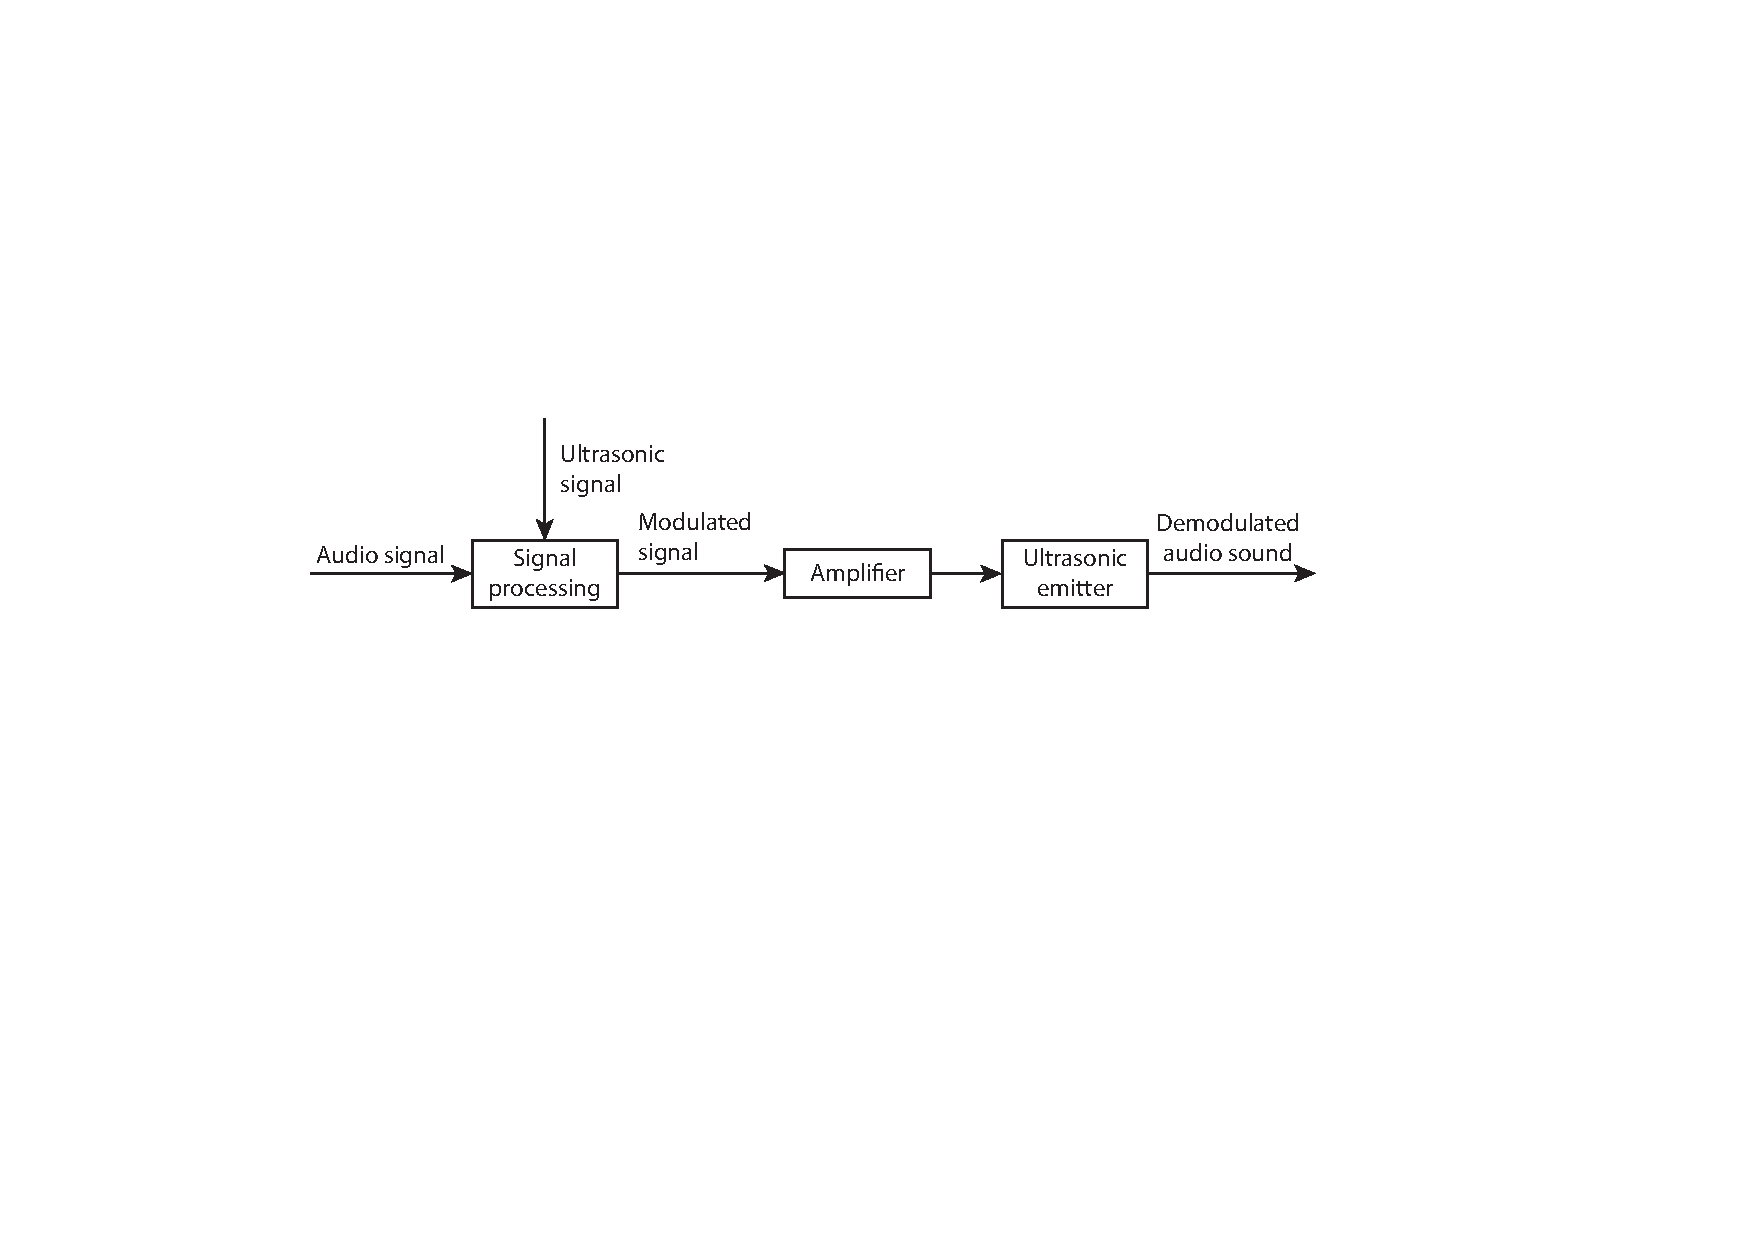
\includegraphics[width = 0.85\textwidth]{fig/Gan2012_PAL_block_diagram/Gan2012_PAL_block_diagram.pdf}
    \caption{Block diagram of the implementation of a PAL. From Fig.~11 of \cite{Gan2012ReviewParametricAcoustic}.}
    \label{fig:Gan2012AA:block_diagram}
\end{figure}
% 考虑是否加入传统换能器的对比
\paragraph{Ultrasonic emitter}\mbox{}\\
The piezoelectric transducers are the most common ultrasonic emitters used in PALs. 
Table~\ref{tab:eifsdf} and Fig.~\ref{fig:flksdafsdf} present some commercial emitters.
It is found the emitter type MA40S4S from Murata is the most popular one.

\begin{table}
    \centering
    \begin{tabular}{cccc}
        \toprule
        Model & Company & \makecell{Center frequency} & Used in \\
        \midrule
        Airducer AT-50 & AirMar & 50 kHz & \cite{Hedberg2010SelfsilencedSoundBeam, Johnson2016ModulationRadioFrequency}\\
        Airducer AT-75 & AirMar & 75 kHz & \cite{Hedberg2010SelfsilencedSoundBeam}\\
        FBULS1007P-T & Ningbo Best Group Factory & 40 kHz& \cite{Marzo2017TinyLevMultiemitterSingleaxis}\\
        MA40H1S-R & Murata & 40 kHz & \cite{Jager2019AirborneUltrasoundPhased}\\
        MA40S4S & Murata & 40 kHz& \cite{Marzo2017TinyLevMultiemitterSingleaxis, Hahn2021ParametricArrayUsing, Jager2019AirborneUltrasoundPhased, Marzo2017UltrainoOpenPhasedarray,Sayin2013RealizationOmnidirectionalSource, Sayin2013DirectivityControlEfficiency, Ji2019ExperimentalInvestigationParameters, Shi2013InvestigationSteerableParametric, Tseng2018PhasedArrayFocusing, Hirayama2019VolumetricDisplayVisual}\\
        MCUSD16A40S12RO & MultiComp & 40 kHz& \cite{Marzo2017TinyLevMultiemitterSingleaxis}\\
        MCUST10P40B07RO & MultiComp & 40 kHz& \cite{Marzo2017TinyLevMultiemitterSingleaxis, Arnela2018ConstructionOmnidirectionalParametric, Arnela2021CharacterizationOmnidirectionalParametric}\\
        MSO-A1625H12T & Manorshi & 25 kHz & Not found\\
        MSO-P1640H10TR &  Manorshi & 40 kHz& \cite{Marzo2017TinyLevMultiemitterSingleaxis}\\
        MSO-A1640H10T & Manorshi & 40 kHz& \cite{Marzo2017TinyLevMultiemitterSingleaxis}\\
        MSO-P1040H07T & Manorshi & 40 kHz& \cite{Marzo2017TinyLevMultiemitterSingleaxis}\\
        T4010B4 & Nippon Ceramic & 40 kHz & \cite{Ochiai2017HolographicWhisperRendering}\\
        ZT40-16 & Shanghai Nicera Sensor & 40 kHz & \cite{Ji2016DevelopmentAcousticFilter, Ji2019ExperimentalInvestigationParameters}\\
        \bottomrule
    \end{tabular}
    \caption{Commercial ultrasonic emitters.}
    \label{tab:eifsdf}
\end{table}

\begin{figure}[!htb]
    \centering
    \begin{subfigure}{0.3\textwidth}
        \centering
        \includegraphics[width = \textwidth]{fig/20211226022137_resize.png}
        \caption{Murata MA40S4S. From Fig.~2.17(a) in \cite{Jager2019AirborneUltrasoundPhased}. }
    \end{subfigure}
    \qquad
    \begin{subfigure}{0.3\textwidth}
        \centering
        \includegraphics[width = \textwidth]{fig/20211226022344_resize.png}
        \caption{Murata MA40H1S-R. From Fig.~2.17(b) in \cite{Jager2019AirborneUltrasoundPhased}. }
    \end{subfigure}
    \caption{Commercial ultrasonic emitters.}
    \label{fig:flksdafsdf}
\end{figure}

The electroacoustic efficiency is usually very low for traditional ultrasonic emitters. 
The main reason is the large acoustic impedance mismatch between air ($\SI{415}{Rayls}$) and the emitter (e.g., $\SI{34}{MRayls}$ for PZT4) \cite{Gallego-Juarez1978UltrasonicTransducerHigh}.
A promising approach is to reduce the characteristic mechanical impedance of the emitter by using a {thin-film} structure, which can be fabricated using the micromachined technique \cite{Lee2009MicromachinedSourceTransducer}.
Piezoelectric micromachined ultrasonic transducers (PMUTs) are compact and efficient emitters for PALs .
Lee et al.\ designed and fabricated a PMUT and the electroacoustic efficiency is measured {to be} 21.9\% \cite{Lee2009MicromachinedSourceTransducer}.
Later, they improved the efficiency to 58.4\% \cite{Je2013ImpactMicromachinedUltrasonic} and {then} 71\% \cite{Je2015MicromachinedEfficientParametric}.
Furthermore, the PMUT has a wide bandwidth, and a $\pm\SI{3}{dB}$ bandwidth of 17 kHz was reported for the ultrasonic waves \cite{Je2015MicromachinedEfficientParametric}.


\paragraph{Power amplifier}\mbox{}\\
The class D amplifier is usually used due to its high efficiency in electroacoustic conversion \cite{Stark2007DirectDigitalPulse}.
Early implementation of PALs use{d} analog circuits, see \cite{Pompei2002SoundUltrasoundParametric} for example. 
Modern PALs are adopting digital circuits, where the digital signal processor (DSP) and field programmable gate array (FPGA) are usually used as the signal processor. 
Karnapi et al.\ designed and implemented a PAL system in FPGA platform using the Altera 1S10 device \cite{Karnapi2004FPGAImplementationParametric}.
{
    Recently, the metal-oxide-semiconductor field-effect transistor (MOSFET) is introduced to amplify the ultrasonic emitters \cite{Marzo2017UltrainoOpenPhasedarray, Hahn2021ParametricArrayUsing}. 
    In 2021, a phased array PAL was realized by Hahn et al.\ using a microcontroller and MOSFET drivers \cite{Hahn2021ParametricArrayUsing}. 
    It is showed that the switching mechanism of the MOSFETs benefit to the signal processing and steering the sound beam.
}

\paragraph{Signal processing methods}\mbox{}\\
The audio signal cannot be radiated by the ultrasonic emitter directly, {as} it has to be modulated into ultrasonic signals via signal processors.
A fundamental preprocessing technique is the amplitude modulation, which is usually called the double sideband (DSB) amplitude modulation in {the literature} \cite{Yoneyama1983AudioSpotlightApplication}.
However, the lower and upper sideband introduced in the DSB amplitude modulation suffer from interference which causes distrotions. 
The single sideband (SSB) modulation method was proposed, where a quadrature path is used to cancel the nonlinear distortion \cite{Aoki1991ParametricLoudspeakerCharacteristics}. 
Kamakura et al.\ proposed the square root (SRT) modulation method in 1984, which can be used to eliminate all of the undesired harmonics theoretically \cite{Kamakura1984DevelopmentsParametricLoudspeaker}.
However, the SRT modulation method requires an ideal ultrasonic emitter that has a perfect flat response (i.e., infinite bandwidth to produce the square-root), which is impossible in real implementations \cite{Shi2016EffectUltrasonicEmitter}.
The effects of the ultrasonic emitter on the distortion performance for different modulation methods {are} compared and reviewed in \cite{Shi2016EffectUltrasonicEmitter}.
A more practical technique called modifield amplitude modulation was proposed based on the quadrature amplitude modulation \cite{Gan2008DistortionAnalysisReduction, Tan2010PreprocessingTechniquesBandlimited, Ji2010TheoreticalExperimentalComparison, Tan2010PreprocessingTechniquesBandlimited}.

In addition to the efforts on eliminating the harmonic distortion, 
signal processing techniques are used to equalize the frequency response of the PAL.
According to the Berktay's far field solution \cite{Berktay1965PossibleExploitationNonlinear}, there is a decrement of 12 dB/octave in the frequency response of the audio sound generated by a PAL \cite{Yoneyama1983AudioSpotlightApplication}.
In 1998, Kite et al.\ proposed a method to equalize by introducing a double integral \cite{Kite1998ParametricArrayAir}.
More concerns are focuesd on the virtual bass enhancement, which is a psychoacoustic signal processing technique enhancing the low frequency sound by adding the harmonics of the fundamental frequency \cite{Arora2006LowComplexityVirtual, Karnapi2002MethodEnhanceLow, Gan2010AudioProjectionDirectional, Shi2013PsychoacousticalPreprocessingTechnique}. 

\paragraph{Applications and commercial products}\mbox{}\\
The PAL has attracted much attention in audio applications because of its sharp directivity, small size, and negligible sidelobes compared to the traditional loudspeakers.
Due to these advantages, PALs have been widely used in applications including ANC systems \cite{Tanaka2010ActiveNoiseControl, Tanaka2011MathematicallyTrivialControl, Tanaka2014MultichannelActiveNoise, Tanaka2017BinauralActiveNoise}, 
personal communications \cite{Nakashima2005PrototypeParametricArray}, 
museum exhibitions and service and multimedia booths \cite{Kortbek2008CommunicatingArtInteractive}, 
measurement of the acoustic parameters of materials \cite{Castagnede2006ReflectionTransmissionNormal, Castagnede2008LowFrequencySitu}, 
mobile robotic navigation \cite{Skinner2019DemonstrationLengthLimited},
stand-off concealed weapons detection \cite{Rudd2008SimulationIncidentNonlinear},
directivity control \cite{Shi2014OverviewDirectivityControl}, 
constructions of omnidirectional loudspeakers \cite{Arnela2018ConstructionOmnidirectionalParametric, Arnela2021CharacterizationOmnidirectionalParametric},
sound reproduction systems \cite{Alunno2017DirectionalLandscapesUsing};
and many other areas.
The applications of PALs in ANC systems will be introduced in detail in Sec.~\ref{sec:review_anc_pal}.
{Due to its potential in audio applications, some commercial PALs are available on the market and presented in Table \ref{tab:pal_commercial_product} and Fig.~\ref{fig:pal_commercial_product}.
}

\begin{table}[H]
    \centering
    \begin{tabular}{lll}
        \toprule
        Model & Company & Country\\
        \midrule
        Audio Spotlight & Holosonics & USA \\
        Hypersound & Turtle Beach Corporation& France\\
        MSP-50E & Mistubishi Electric Engineering Company & Japan\\
        Acouspade speaker &  Ultrasonic Audio Technologies& Slovenia\\
        Focusound directional speaker & Audfly Technology (Suzhou) & China \\
        Soundlazer & Richard Haberkern & USA\\
        \bottomrule
    \end{tabular}
    \caption{Commercial products of the PAL.}
    \label{tab:pal_commercial_product}
\end{table}
\begin{figure}[!htb]
    \centering
    \begin{subfigure}{0.3\textwidth}
        \centering
        \includegraphics[width=\textwidth]{fig/CommercialProducts/As-24i.png}
        \caption{Audio Spotlight AS-24i from \cite{HolosonicsAudioSpotlight24i}}
    \end{subfigure}
    \hfill
    \begin{subfigure}{0.3\textwidth}
        \centering
        \includegraphics[width=\textwidth]{fig/CommercialProducts/Hypersound_resize.png}
        \caption{HyperSound HSS3000 from \cite{TurtleBeachCorporationHyperSoundHSS300}}
    \end{subfigure}
    \hfill
    \begin{subfigure}{0.2\textwidth}
        \centering
        \includegraphics[width=\textwidth]{fig/CommercialProducts/MSP-50E_resize.png}
        \caption{MST-50E from \cite{MitsubishiElectricMSP050E}}
    \end{subfigure}
    \\
    \begin{subfigure}{0.35\textwidth}
        \centering
        \includegraphics[width=\textwidth]{fig/CommercialProducts/Acouspade-directional-Sound-Speaker_resize.jpg}
        \caption{Acouspade from \cite{UltrasonicAudioTechnologiesACOUsticSPAceDElimiter}}
    \end{subfigure}
    \hfill
    \begin{subfigure}{0.3\textwidth}
        \centering
        \includegraphics[width=\textwidth]{fig/CommercialProducts/FocusoundModelR.jpg}
        \caption{Focusound Model R from \cite{2021ProductsDescriptionsFocusound}}
    \end{subfigure}
    \hfill
    \begin{subfigure}{0.2\textwidth}
        \centering
        \includegraphics[width=\textwidth]{fig/CommercialProducts/Soundlazer_resize.png}
        \caption{Soundlazer SL-01 from \cite{2021SoundlazerPuttingSound}}
    \end{subfigure}
    \caption{Several commercial products of the PAL.}
    \label{fig:pal_commercial_product}
\end{figure}

% The earliest applications for PAAs lie in sonar \cite{Berktay1965ParametricAmplificationUse, Browning2009ParametricAcousticArray, Ostrovsky2009ResearchParametricArrays}.

%----------------------------------------------------------------------------------------
%	SECTION 2
%----------------------------------------------------------------------------------------

\section{Active noise control (ANC)}
\label{sec:review_anc}

Lueg {was the first to introduce} the concept of an ANC system{, which was reported} in a US patent granted in 1936 \cite{Lueg1936ProcessSilencingSound}.
It demonstrated the cancellation of a sound field can be realized by superimposing an electroacoustically generated secondary sound field that has an opposite phase \cite{Lueg1936ProcessSilencingSound, Guicking1990InventionActiveNoise}.
Early ANC applications focused on the control of noise radiated by a transformer \cite{Ross1978ExperimentsActiveControl}.
Nowadays, more and more applications are reported, and the theory and signal processing techniques can be found in textbooks \cite{Nelson1992ActiveControlSound, Fuller1996ActiveControlVibration, Elliott2000SignalProcessingActive, Hansen2012ActiveControlNoise, Kuo1996ActiveNoiseControl}.
In general, there are two types of ANC systems: the global and the local active control.
For a global control system, the aim is to reduce the total radiation from the noise source.
However, it is possible and practical only when the secondary source is close to the noise source (smaller than half of the wavelength) \cite{Nelson1992ActiveControlSound}.
Therefore, local control is more popular which aims to create a small quiet zone at target regions \cite{Joseph1994FieldZonesQuiet}.
This section focuses on the review of {approaches and algorithms to realize an ANC system}, the quiet zone generation, and existing ANC systems using directional loudspeakers and PALs.

\subsection{Approaches and algorithms}
\label{sec:anc_algorithm}
{
Depending on the use of reference sensors, the ANC system can be classified as the feedforward strcture and the feedback structure \cite{Elliott2000SignalProcessingActive}. 
Figure~\ref{fig:anc_structure} shows the feedforward structure of an ANC system, where the reference sensors are placed near the noise source to acquire the primary noise.
The anti-noise control signal emitted by the secondary sources is calculated based on the reference signal.
It goes through the secondary path (the acoustic path from the secondary source and the error point) and entirely cancels the primary nosie at the error sensors.
The residual error signal at error sensors is used to dynamically adjust the output of the control signal enabling the maximum noise reduction. 
\revA{A disadvantage of the feedforward structure is that the reference signal is affected by the sound radiated by the secondary source when the reference signal is recorded by the acoustic based sensors (e.g., microphones)}, which makes the system unstable \cite{Akhtar2007ActiveNoiseControl}.
This can be solved by using directional loudspeakers as secondary sources so that the secondary sound waves do not propgate in the direction of the reference sensors.
Compared to the feedforward strucutre, the feedback structure does not need reference sensors. 
Instead, the information of the primary noise is captured from the error signal.
Although the feedback structure requires less sensors than the feedforward structure, 
it is hard to predict broadband signals due to the limitation of system causility, so it is only used to deal with the narrowband noise \cite{Elliott2000SignalProcessingActive}.
The feedforward ANC is more stable and used in applications, and it is therefore adopted in this thesis.
}

{
% The approach to implementing a feedforward ANC system is to 
It is hard to implement a feedforward ANC system using analog circuits. 
Digital processors with adaptive filter algorithms are generally used nowadays.
The aim of the adaptive filter algorithm in an ANC controller is to find the control filter which enables the maximum noise reduction at error sensors. 
There are various kinds of algorithms to obtain the control filter, while the FxLMS is the most practical one,
and also used in commercial ANC controllers \cite{Shi2020AlgorithmsImplementationsOvercome, Antysound2017TigerANCWiFiQUserManual}.
The mechanism of FxLMS algorithm can be illustrated by Fig.~\ref{fig:98sdjf83j}.
$P(z)$ and $S(z)$ represent the path from the primary noise and secondary srouce to the error point, respectively.
$\hat{S}(z)$ is an estimation of $S(z)$. 
The reference signal denoted by $x(n)$ is filtered by the control filter $W(z)$ and becomes the control signal $y(n)$.
The control filter $W(z)$ is adaptively updated according to the minimize the square of the error signal $e(n)$.
There are also other algorithms to improve the convergence speed and reduce the computational cost of the control filter, such as the normalized FxLMS algorithm \cite{Slock1993ConvergenceBehaviorLMS, Shi2015IdentificationParametricArray}; a more detailed review can be found in \cite{Shi2020AlgorithmsImplementationsOvercome}.
}
\begin{figure}[!htb]
    \centering
    \includegraphics[width = 0.7\textwidth]{fig/shi2019_fxlms.png}
    \caption{Block diagram of the FxLMS algorithm. From Fig.~2.3 in \cite{Shi2020AlgorithmsImplementationsOvercome}.}
    \label{fig:98sdjf83j}
\end{figure}



\subsection{Quiet zone generation}
\label{sec:review_anc_qz}
{The} ANC technique is effective {in controlling a noise source} at the error point. 
However, it only creates a small quiet zone around the error point, and the quiet zone is usually defined as the region where the noise reduction is larger than 10 dB \cite{Elliott2015ModelingLocalActive}. 
Furthermore, the size of the quiet zone becomes smaller as the frequency increases.
For an ANC system with one secondary source, the size of the quiet zone is only about one tenth of the wavelength in a diffuse sound field \cite{Guo1998EffectsReflectiveGround, Elliott1988ActiveCancellationPoint}. 
The challenge to be addressed with ANC involves maximizing the size of {this} quiet zone. 

To enlarge the quiet zone, 
a multi-channel ANC system that has multiple secondary sources and error microphones is usually used  \cite{Zhang2019ActiveNoiseControl}. 
The sound pressure inside a closed surface surrounded by multiple secondary sources can be controlled if the spacing between the secondary sources is sufficiently small \cite{Elliott2018WavenumberApproachAnalysing}. 
In a free field, the quiet zone size is found to be proportional to the number of secondary sources \cite{Guo1997ActivelyCreatedQuiet}.
Experimental measurements show that more than 20 dB of noise reduction can be obtained inside a sphere with a radius of 0.3 m for frequencies from 100 Hz and 500 Hz, when using 30 secondary sources on a spherical surface \cite{Epain2007ActiveControlSound}.
In an ordinary room, experimental results with 16 secondary sources distributed over a cylindrical surface demonstrate that a cylindrical quiet zone with a height of 0.2 m and a radius of 0.2 m is possible below 550 Hz \cite{Zou2007PreliminaryExperimentalStudy}. 
A large quiet zone usually requires a larger number of secondary sources and error microphones, so 
{recent work has focused on} reducing the number of microphones \cite{Maeno2018ModeDomainSpatial} and loudspeakers \cite{Zhang2016MultichannelActiveNoise}. 

In these ANC systems, omnidirectional loudspeakers were used as secondary sources. 
Although the noise inside the target region is reduced, the sound pressure outside the region often increases, which is known as the spillover effect \cite{Guo1997ActivelyCreatedQuiet, Tanaka2010ActiveNoiseControl}. 
{This causes} noise amplification outside the target areas, {which} can be mitigated by optimizing some parameters such as the separation between the secondary sources and the distance between secondary sources and {the} error sensors \cite{Guo1997ActivelyCreatedQuiet, Joseph1994FieldZonesQuiet, David1994NumericalStudiesActively}.
To address this problem, directional loudspeakers have been shown to have the potential to lower this external sound field \cite{Tanaka2010ActiveNoiseControl, Hu2019ActiveCancellationSound}. 
PALs have sharper directivity than most traditional dynamic loudspeakers \cite{Gan2012ReviewParametricAcoustic}, but the feasibility of using them to create a quiet zone is not clear, and so this will be investigated here.

\subsection{ANC using directional loudspeakers}
\label{eq:review_anc_directional}
The type of secondary source in an ANC system is crucial for {delivering high levels of} noise reduction \cite{Bolton1995SoundCancellationUse, Qiu2000SecondaryAcousticSource}.
{It is common for a single monopole, or an array of monopoles, to be used as secondary sources in ANC systems}.
However, directional sources can be used as secondary sources in multiple channel ANC systems to improve performance. 
For example, tripole secondary sources with a cardioid radiation pattern have been used to reduce noise source radiation \cite{Mangiante1977ActiveSoundAbsorption}.
In 2011, Chen et al.\ designed a unidirectional source consisting of two closely located loudspeakers with pre-adjusted phase difference \cite{Chen2011ActiveNoiseBarrier}.
In an active noise barrier (ANB) system as shown in Fig.~\ref{fig:chen2011anb_sketch}, both numerical and experimental results from 160 Hz to 300 Hz have showed that the noise reduction performance can be improved {significantly} by replacing monopole sources with unidirectional sources.
Furthermore, a large quiet zone around the error points was observed \cite{Chen2011ActiveNoiseBarrier}.

\begin{figure}[!htb]
    \centering
    \includegraphics[width = 0.5\textwidth]{fig/chen2011anb_resize.png}
    \caption{Sketch of an ANB system. From Fig.~1(a) of \cite{Chen2011ActiveNoiseBarrier}.}
    \label{fig:chen2011anb_sketch}
\end{figure}

In 2019, Hu and Tang proposed a directional source consisting of a central circular core enclosed within an annulus, as shown in Fig.~\ref{fig:hu2019jasa}(a). 
It has been demonstrated that the proposed source is much more directional {than} a traditional piston source, even {though} its size is much smaller than the latter if the magnitude and the phase of the two parts are optimally designed \cite{Hu2019ActiveCancellationSound}. 
{Hu and Tang used these} directional sources to cancel the noise generated by a finite length coherent line source, as shown in Fig.~\ref{fig:hu2019jasa}(b). 
The numerical results show that the proposed directional sources can make the ANC system more compact and improve noise reduction performance, when compared to traditional piston sources \cite{Hu2019ActiveCancellationSound}.
These directional secondary sources have been chosen because they radiate only in the direction of the target region, and so they have less effect on the other areas reducing the effects of noise amplification outside of the quiet zone.

\begin{figure}[!htb]
    \centering
    \begin{subfigure}{0.3\textwidth}
        \centering
        \includegraphics[width = \textwidth]{fig/hu2019jasa_secondary_source_resize.png}
        \caption{}
    \end{subfigure}
    \begin{subfigure}{0.69\textwidth}
        \centering
        \includegraphics[width = \textwidth]{fig/hu2019jasa_anc_system_resize.png}
        \caption{}
    \end{subfigure}
    \caption{(a) The proposed directional source; (b) a coherent line source of length $l$ is controlled by 3 secondary sources. From Figs.~1 and 5 in \cite{Hu2019ActiveCancellationSound}.}
    \label{fig:hu2019jasa}
\end{figure}

\subsection{ANC using PALs}
\label{sec:review_anc_pal}
% PALs are an application of PAAs in air which can generate highly directional audio sound due to nonlinear interactions of ultrasonic waves.
% Therefore, PALs are a promising secondary source, and several attempts have been made to employ them in ANC systems. 
% {PALs have been used as secondary sources in ANC systems to improve the noise reduction performance. }
In 2005, Brooks et al.\ was the first to investigate the feasibility of using PALs in ANC systems as secondary sources \cite{Brooks2005InvestigationFeasibilityUsing}.
They pointed out two concerns in practical applications which might adversely affect the performance of such an ANC system.
The first is that the frequency response of a PAL is poor at low frequencies, so that the noise reduction performance would deteriorate significantly as the frequency decreases.
The second is that the demodulated audio sound in air is found to vary quickly as a function of time, so that the performance controlling \revA{wideband} noise would be degraded.
{
It is noted that the low frequency response of PALs may be improved by focusing the sound beams \cite{Lucas1983FieldParametricFocusing, Saito1986SimpleAnalyticalModel, Saito1998ExperimentParametricFocusing, Cervenka2021ParametricAcousticArray}.
}

The quiet zone is usually generated around a fixed error microphone for ANC systems. 
To overcome this limitation, Kidner et al.\ proposed an ANC system using PALs to create a moving local quiet zone with the aid of virtual sensing techniques, as shown in Fig.~\ref{fig:kidner2006_sketch} \cite{Kidner2006FeasibilityStudyLocalised}.
Their results showed that the quiet zone created by the PAL can be extended further in the radial direction {when compared to} a traditional piston source. 
The reason is that the sound wave generated  by a PAL decays slowly resulting in a better matching between the primary (noise) and secondary sound fields.

\begin{figure}[!htb]
    \centering
    \includegraphics[width = 0.4\textwidth]{fig/kidner2006fig1_resize.png}
    \caption{Illustration of the concept of a directional control source (PAL, denoted by \quotes{Spotlight}) being used in combination with a virtual sensor to allow tracking of a local quiet zone, without spillover in the rest of the field. The shaded area shows the region that is affected by the secondary source. From Fig.~1 of \cite{Kidner2006FeasibilityStudyLocalised}.}
    \label{fig:kidner2006_sketch}
\end{figure}

Despite the advantages of using PALs in ANC systems, the target point is limited along the radiation direction of the PAL due to its sharp directivity. 
To cope with this problem, a steerable PAL employing the phased array technique was proposed by Tanaka and Tanaka in 2010 \cite{Tanaka2010ActiveNoiseControl}.
As shown in Fig.~\ref{fig:tanaka2010jasa_steer30}, the noise at an error point (denoted by circle markers) in the $30^\circ$ direction can be reduced by a secondary source (denoted by square markers) at the origin.
Both numerical and experimental results show similar noise reduction performance can be achieved around the error point, but the noise amplification (spillover effect) in the {surrounding} areas is negligible for the case with a PAL.
This successful realization of the steerable PAL is an attractive technique for tracking control of a moving target without mechanically rotating the PAL, as shown in Fig.~\ref{fig:kidner2006_sketch}.

\begin{figure}[!htb]
    \centering
    \begin{subfigure}{0.4\textwidth}
        \centering
        \includegraphics[width = \textwidth]{fig/tanaka2010jasa_fig11_resize.png}
    \end{subfigure}
    \begin{subfigure}{0.4\textwidth}
        \centering
        \includegraphics[width = \textwidth]{fig/tanaka2010jasa_fig12_resize.png}
    \end{subfigure}
    \caption{Sound fields steered by \ensuremath{30^\circ}.  
        \revA{Left column, numerical results; right column, experimental results; 
        top row, before control; 
        middle row, after control using a traditional loudspeaker;
        bottom row, after control using a PAL.}
    Cross, noise source; Square, secondary source; Circle, error point. 
From Figs.~11 and 12 in \cite{Tanaka2010ActiveNoiseControl}.}
    \label{fig:tanaka2010jasa_steer30}
\end{figure}

Tanaka and Tanaka continued their work and proposed a focused PAL, shown in Fig.~\ref{fig:tanaka20112309f}, to achieve a mathematically trivial global control of the sound radiated by a point source \cite{Tanaka2011MathematicallyTrivialControl}. 
The {measured and predicted} audio sound pressure is shown in Fig.~\ref{fig:tanaka2011we90fsf}. 
It is well known that the global control is very limited when the separation of the primary and secondary sources is larger than the half of the wavelength, which is 0.17 m at 1 kHz \cite{Nelson1992ActiveControlSound}.
However, they claim global control is observed when using a focused PAL even {when} the distance between primary and secondary sources (0.3 m in Fig.~\ref{fig:tanaka20112309f}) is larger than {half of wavelength}.
It should be noted that the trivial method is hard to realize in applications, and the performance for broadband noise still needs to be investigated.
The global sound power control using PALs in an ANC system has also been investigated numerically by Ye et al.\ \cite{Ye2012ActivelyCreatedQuiet}. 
They developed a framework to analyze the sound power output by a PAL in ANC systems.
A useful conclusion is that {the} minimization of the total power output of the system is the same as the minimization of the power output only by the PAL, due to its sharp directivity.
However, it should be noted that the power output of the PAL is calculated based on a far field solution in \cite{Ye2012ActivelyCreatedQuiet}, which is rather inaccurate.

\begin{figure}[!htb]
    \centering
    \includegraphics[width = 0.7\textwidth]{fig/tanaka2011fig4_resize}
    \caption{The laboratory made focused PAL in \cite{Tanaka2011MathematicallyTrivialControl}.}
    \label{fig:tanaka20112309f}
\end{figure}
\begin{figure}[!htb]
    \centering
    \begin{subfigure}{0.4\textwidth}
        \centering
        \includegraphics[width = \textwidth]{fig/tanaka2011fig3_resize.png}
    \end{subfigure}
    \begin{subfigure}{0.4\textwidth}
        \centering
        \includegraphics[width = \textwidth]{fig/tanaka2011fig8_resize.png}
    \end{subfigure}
    \caption{Simulation (left column) and measurement (right column) audio sound pressure of locally global noise control at 1 kHz: 
        (top row) before control, (middle row) after control with the focused PAL, and (bottom) after control with an ideal point source. 
    Cross mark, primary source; square mark, secondary source; circle mark, error point.
    From Figs.~3 and 8 in \cite{Tanaka2011MathematicallyTrivialControl}.
}
    \label{fig:tanaka2011we90fsf}
\end{figure}


Except for the ANC systems used in free field, the PAL has also been used to cancel the noise in a room \cite{Ganguly2014RealtimeRemoteCancellation}.
As shown in Fig. \ref{fig:ganguly2014}, a commercial PAL (Audio Spotlight AS-24i \cite{HolosonicsAudioSpotlight24i}) is used as a secondary source in an ANC system. 
Contrary to the aforementioned literatures, an adaptive ANC algorithm (leaky normalized least mean square) was used, so that the \revA{wideband} noise can be reduced adaptively.

\begin{figure}[!htb]
    \centering
    \includegraphics[width = 0.6\textwidth]{fig/ganguly2014fig5_resize.png}
    \caption{Experimental setup of an ANC system using a commercial PAL in a room. From Fig.~5 in \cite{Ganguly2014RealtimeRemoteCancellation}.}
    \label{fig:ganguly2014}
\end{figure}

Later, PALs {have been} extended to the multi-channel ANC systems. 
{For example, in} 2017 a two-channel ANC system using PALs was proposed to reduce the binaural factory noise at human ears \cite{Tanaka2017BinauralActiveNoise}, and the sketch is shown in Fig.~\ref{fig:intro:tanaka2017model}.
{This} demonstrated two advantages of using PALs in multi-channel ANC systems.
First, the noise at target points can be reduced while the sound pressure in other areas is not affected.
Second, the crosstalk between secondary paths is negligible so the crosstalk cancellation technique is not required. 
As shown in Fig.~\ref{fig:tanaka_2017_results}, it is clear that the noise reduction performance without the crosstalk cancellation is almost the same as that with the crosstalk.

\begin{figure}[!htb]
    \centering
    \begin{subfigure}{0.475\textwidth}
        \centering
        \includegraphics[width = \textwidth]{fig/tanaka2017_1660x1120a.png}
        \caption{Left ear}
    \end{subfigure}
    \begin{subfigure}{0.475\textwidth}
        \centering
        \includegraphics[width = \textwidth]{fig/tanaka2017_1660x1120b.png}
        \caption{Right ear}
    \end{subfigure}
    \caption{Experiment results of the dual-channel ANC system that achieves 10.4 dB and 11.6 dB noise reductions at the left and right ears, respectively. From Fig.~8 in \cite{Tanaka2017BinauralActiveNoise}.}
    \label{fig:tanaka_2017_results}
\end{figure}


The length-limited PAL has also been used for ANC.
Shi and Gan proposed a theoretical framework based on the KZK equation for a length-limited PAL that has a concentrically-nested structure to cancel the noise in an ANC system \cite{Shi2013UsingLengthlimitedParametric}.
The length-limited PAL is shown in Fig.~\ref{fig:length_limited_PAL_Lam2014}.
The speaker is made up of an inner hexagonal array of 36 emitters with {a} center frequency of 40 kHz, and an outer annulus of 36 emitters with {a} center frequency of 25 kHz.
Based on this framework, Lam et al.\ investigated the feasibility of using a length-limited PAL in an ANC system \cite{Lam2014FeasibilityLengthlimitedParametric}.
Their experimental results show that a noise source at 1.5 kHz in a pipe is reduced by 18.4 dB at 8 m using such a length-limited PAL.
A preliminary numerical study on the formation of a quiet zone using length-limited PAL is also presented in \cite{Wang2019FormationLocalQuiet}. 

\begin{figure}[htb]
    \centering
    \includegraphics[width = 0.4\textwidth]{fig/length_limited_PAL_Lam2014_resize.png}
    \caption{A concentrically-nested length-limited PAL made for ANC. From Fig. 2 in \cite{Lam2014FeasibilityLengthlimitedParametric}.}
    \label{fig:length_limited_PAL_Lam2014}
\end{figure}



\section{Summary}
This chapter presents a literature review on the PAL and ANC systems in Secs.~\ref{sec:literature_pal} and \ref{sec:review_anc}, respectively.
In Sec.~\ref{sec:literature_pal_phys}, the physical mechanisms and fundamental properties of audio sound generated by a PAL are introduced. 
Section \ref{sec:review_pal_predict} {then} reviews existing prediction models, which include the quasilinear approximation, the far field solution, and the governing equations.
The implementation and applications of PALs, including commercial products, are presented in Sec.~\ref{sec:review_implement}.
The approaches and algorithms to realize an ANC system are introduced in Sec.~\ref{sec:anc_algorithm}.
In Sec.~\ref{sec:review_anc_qz}, the ANC system for the purpose of the generation of a quiet zone is surveyed. 
Section \ref{eq:review_anc_directional} focuses on the ANC system using directional loudspeakers and Sec.~\ref{sec:review_anc_pal} reviews the existing work on ANC using PALs.

% Based on the literature review, the following research questions are identified:
% \begin{outline}
    % % \1 The prediction models based on the Westervelt and Kuznetsov equations require an evaluation of five-fold integrals under the quasilinear assumption. 
    % % Is it possible to develop a method to simplify the calculation without minimizing the effects on the prediction accuracy?
    % % \1 There are applications when the PAL is non-baffled, but existing models are not applicable for predicting the audio sound on the back side. 
    % % How to develop a theoretical model to predict the audio sound on the back side of a non-baffled PAL?
    % % \1 The audio sound generated by a PAL can be treated as the superposition of the sound generated by infinitely many virtual sources in space with the source density proportional to the product of the ultrasound pressure. 
    % % Therefore, the formation of the audio sound is accumulated before the ultrasound being totally absorbed in air. 
    % % It is interesting to know what would happen if such an accumulation process is truncated by a reflecting surface, blocked by a partition, or scattered by a sphere.
    % % \1 The advantages of using PALs in ANC systems have been demonstrated in existing literatures. 
    % % However, it is necessarily to know if a large quiet zone can be created by multiple PALs and if it is possible to cancel a broadband noise for PALs.
    % \1  {
    % The advantages of using PALs in ANC systems have been demonstrated in existing studies. 
    % Most of existing studies focus on using one or two PALs to cancel the narrow band noise at error points. 
    % However, the generated quiet zone is rather small. 
    % It is necessary to know if a large quiet zone can be created by multiple PALs and if it is possible to cancel a broadband noise for PALs. }
    % \1 {
        % Heavy computations are required in a multi-channel ANC system due to a large number of PALs. 
        % The prediction accuracy 
    % }
% \end{outline}
